%%%%%%%%%%%%%%%%%%%%%%%%%%%%%%%%%%%%
%                                  %
% Titre  : s_p.tex                 %
% Sujet  : Manuel de l'utilisateur %
%          du projet 'Scotch'      %
%          Programmes              %
% Auteur : Francois Pellegrini     %
%                                  %
%%%%%%%%%%%%%%%%%%%%%%%%%%%%%%%%%%%%

\section{Programs}
\label{sec-prog}

The programs of the \scotch\ project belong to five distinct classes.
\begin{itemize}
\item
Graph handling programs, the names of which begin in ``\texttt{g}'',
that serve to build and test source graphs.
\item
Mesh handling programs, the names of which begin in ``\texttt{m}'',
that serve to build and test source meshes.
\item
Target architecture handling programs, the names of which begin
in ``\texttt{a}'', that allow the user to build and test decomposition-defined
target files, and especially to turn a source graph file into a target file.
\item
The mapping and ordering programs themselves.
\item
Output handling programs, which are
the mapping performance analyzer, the graph factorization program,
and the graph, matrix, and mapping visualization program.
\end{itemize}
The general architecture of the \scotch\ project is displayed in
Figure~\ref{fig-synp}.

\begin{figure}[p]
\centering{\hspace*{-5em}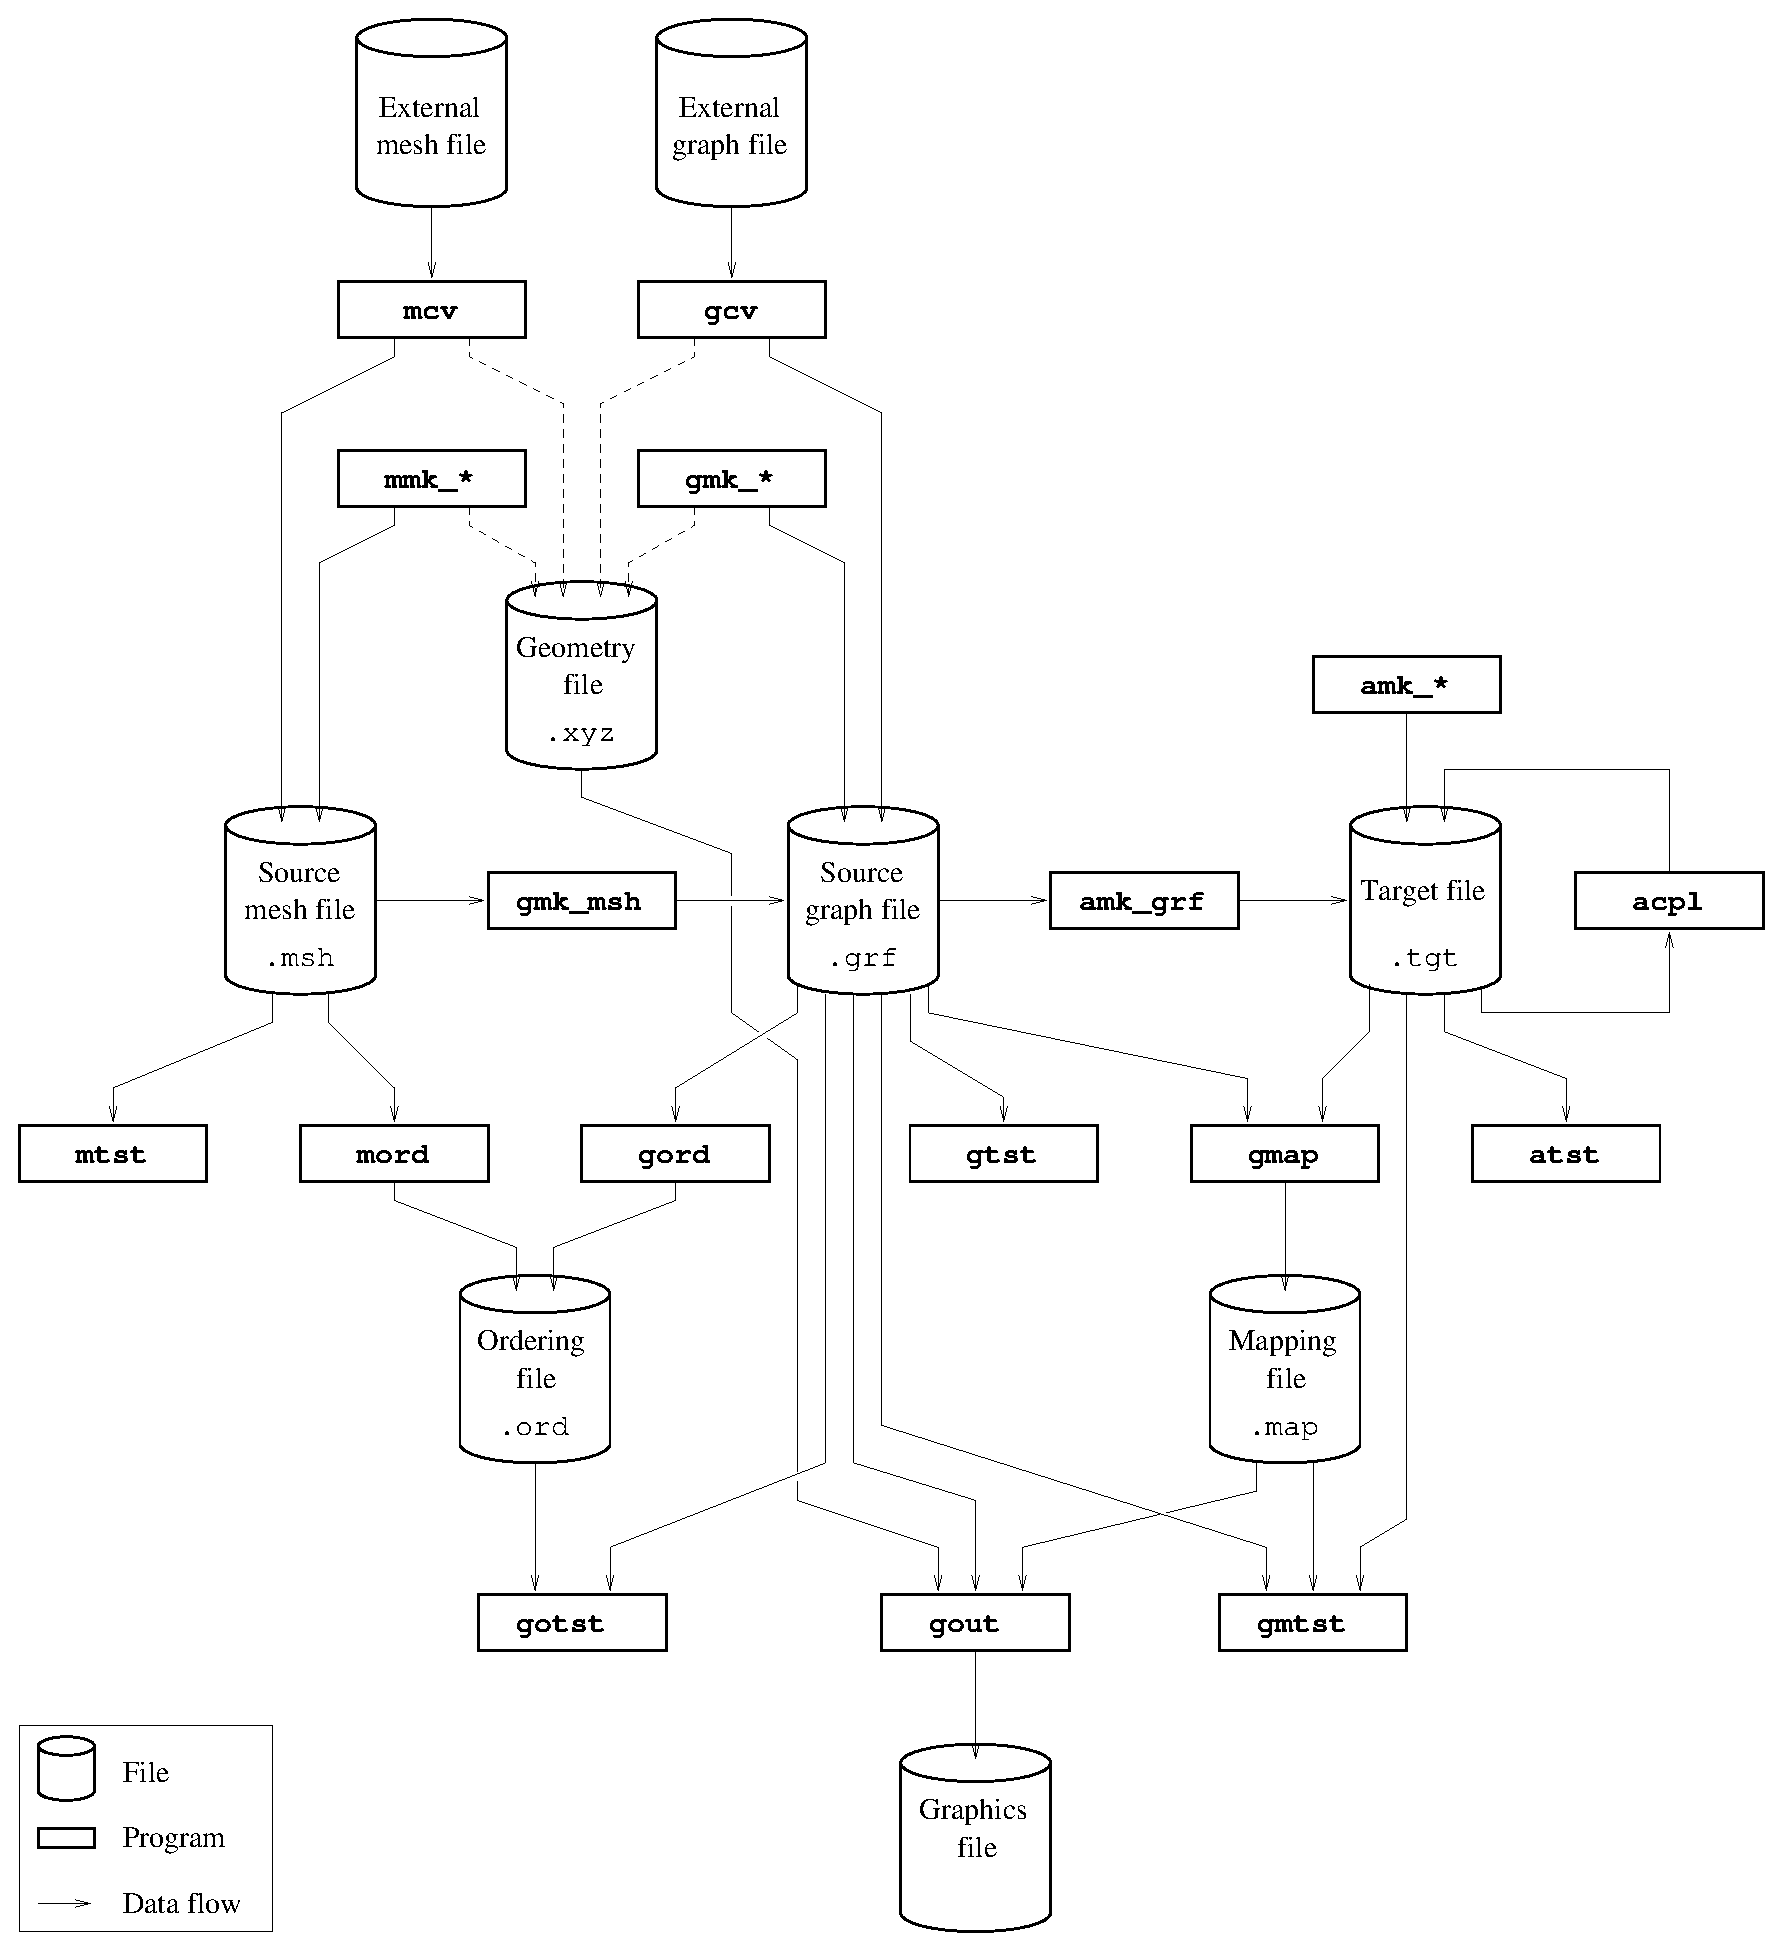
\includegraphics[scale=0.56]{s_f_synp.eps}}
\caption{General architecture of the \scotch\ project. All of the
features offered by the stand-alone programs are also available in
the \libscotch\ library.}
\label{fig-synp}
\end{figure}

\subsection{Invocation}

The programs comprising the \scotch\ project have been designed to run in
command-line mode without any interactive prompting,
so that they can be called easily from other programs by means of
``\mbox{\texttt{system$\,$()}}'' or ``\mbox{\texttt{ popen$\,$()}}''
system calls, or be piped together on a single shell command line. In
order to facilitate this, whenever a stream name is asked for (either
on input or output), the user may put a single ``\texttt{-}'' to
indicate standard input or output. Moreover, programs read their input
in the same order as stream names are given in the command line. It
allows them to read all their data from a single stream (usually the
standard input), provided that these data are ordered properly.

A brief on-line help is provided with all the programs. To get this help,
use the ``\texttt{-h}'' option after the program name.
The case of option letters is not significant, except when
both the lower and upper cases of a letter have different meanings.
When passing parameters to the programs, only the order of file names is
significant; options can be put anywhere in the command line, in any order.
Examples of use of the different programs of the \scotch\ project are provided
in section~\ref{sec-examples}.

Error messages are standardized, but may not be fully explanatory.
However, most of the errors you may run into should be related to file
formats, and located in ``\mbox{\texttt{ \ldots Load}}'' routines.
In this case, compare your data formats with the definitions
given in section~\ref{sec-file}, and use the \texttt{gtst} and \texttt{mtst}
programs to check the consistency of source graphs and meshes.

\subsection{Using multi-threading}
\label{sec-prog-multithread}

Starting from version \textsc{6.1.0}, thread management in \scotch\ is
dynamic. This allows the user to control dynamically the number of
threads that are used by the threaded algorithms of the
\libscotch\ library and, consequently, by the \scotch\ standalone
programs that call them. These algorithms are enabled when \scotch\ is
compiled with the flag ``\texttt{-DSCOTCH\_\lbt PTHREAD}'' set.

Unless explicitly prevented to do so, \scotch\ standalone programs
will detect the number of cores available on the user's system and
will use as many of them as prescribed at compile time or, if no upper
threshold was set at that time, all of those which are currently
available. This behavior can be controlled further by means of the
shell environment variable
``\texttt{SCOTCH\_\lbt PTHREAD\_\lbt NUMBER=}$x$'', where $x$ is the
prescribed maximum number of threads to be used. Setting a thread
number to $1$ will coerce \scotch\ into using only purely sequential
algorithms (which may differ in nature from their multi-threaded
counterparts). Setting the thread number to $-1$ will make
\scotch\ use all available cores, overriding the value possibly set at
compile time.

\subsection{Using compressed files}
\label{sec-prog-compressed}

Starting from version {\sc 5.0.6}, \scotch\ allows users to provide
and retrieve data in compressed form. Since this feature requires that
the compression and decompression tasks run in the same time as data
is read or written, it can only be done on systems which support
multi-threading (Posix threads) or multi-processing (by means of
\texttt{fork} system calls).

To determine if a stream has to be handled in compressed form,
\scotch\ checks its extension. If it is ``\texttt{.gz}'' (\texttt{gzip}
format), ``\texttt{.bz2}'' (\texttt{bzip2} format) or ``\texttt{.lzma}''
(\texttt{lzma} format), the stream is assumed to be compressed according
to the corresponding format. A filter task will then be used to process
it accordingly if the format is implemented in \scotch\ and enabled on
your system.

To date, data can be read and written in \texttt{bzip2} and \texttt{gzip}
formats, and can also be read in the \texttt{lzma} format. Since the
compression ratio of \texttt{lzma} on \scotch\ graphs is $30\%$ better
than the one of \texttt{gzip} and \texttt{bzip2} (which are almost
equivalent in this case), the \texttt{lzma} format is a very good choice
for handling very large graphs. To see how to enable compressed data
handling in \scotch, please refer to Section~\ref{sec-install}.
\\

When the compressed format allows it, several files can be provided on
the same stream, and be uncompressed on the fly. For instance, the
command ``\texttt{cat brol.grf.gz brol.xyz.gz | gout -.gz -.gz -Mn -
brol.iv}'' concatenates the topology and geometry data of some graph
\texttt{brol} and feed them as a single compressed stream to the standard
input of program \texttt{gout}, hence the ''\texttt{-.gz}'' to indicate a
compressed standard stream.

\subsection{Description}

\subsubsection{\texttt{acpl}}

\begin{itemize}
\progsyn
\texttt{acpl} [{\it input\_target\_file} [{\it output\_target\_file}]] {\it options}

\progdes
The program \texttt{acpl} is the decomposition-defined architecture file compiler.
It processes architecture files of type ``\texttt{deco~0}'' built by hand or by
the \texttt{amk\_}* programs, to create a ``\texttt{deco~1}'' compiled
architecture file of about four times the size of the original one;
see section~\ref{sec-file-target-deco}, page~\pageref{sec-file-target-deco},
for a detailed description of decomposition-defined target
architecture file formats.
\\
The mapper can read both original and compiled architecture file formats.
However, compiled architecture files are read much more efficiently, as
they are directly loaded into memory without further processing.
Since the compilation time of a target architecture graph evolves
as the square of its number of vertices, precompiling with \texttt{acpl} can
save some time when many mappings are to be performed onto the same large
target architecture.

\progopt
\begin{itemize}
\iteme[\texttt{-h}]
Display the program synopsis.
\iteme[\texttt{-V}]
Print the program version and copyright.
\end{itemize}
\end{itemize}

\subsubsection{\texttt{amk\_}*}
\relax
\begin{itemize}
\progsyn
\texttt{amk\_ccc} {\it dim} [{\it output\_target\_file}] {\it options}\\
~\\
\texttt{amk\_fft2} {\it dim} [{\it output\_target\_file}] {\it options}\\
~\\
\texttt{amk\_hy} {\it dim} [{\it output\_target\_file}] {\it options}\\
~\\
\texttt{amk\_m2} {\it dimX} [{\it dimY} [{\it output\_target\_file}]] {\it options}\\
~\\
\texttt{amk\_p2} {\it weight0} [{\it weight1} [{\it output\_target\_file}]] {\it options}\\

\progdes
The \texttt{amk\_}* programs make target graphs.
Each of them is devoted to a specific topology, for which it builds target
graphs of any dimension.
\\
These programs are an alternate way between algorithmically-coded
built-in target architectures and decompositions computed by mapping
with \texttt{amk\_grf}.
Like built-in target architectures, their decompositions are
algorithmically computed, and like \texttt{amk\_grf}, their output is
a decomposition-defined target architecture file.
These programs allow the definition and testing of new algorithmically-coded
target architectures without coding them in the core of the mapper.
\\

\noi
Program \texttt{amk\_ccc} outputs the target architecture file of a
Cube-Connected-Cycles graph of dimension {\it dim}.
Vertex $(l,m)$ of $\CCC(dim)$, with $0 \leq l < dim$ and $0 \leq m < 2^{dim}$,
is linked to vertices $((l-1) \bmod dim, m)$, $((l+1) \bmod dim,m)$, and
$(l, m \oplus 2^l)$, and is labeled $l\times 2^{dim} + m$. $\oplus$ denotes
the bitwise exclusive-or binary operator, and $a \bmod b$ the integer
remainder of the euclidian division of $a$ by $b$.
\\

\noi
Program \texttt{amk\_fft2} outputs the target architecture file of a
binary Fast-Fourier-Transform graph of dimension {\it dim}.
Vertex $(l,m)$ of $\FFT(dim)$, with $0 \leq l \leq dim$ and
$0 \leq m < 2^{dim}$, is linked to vertices
$(l-1, m)$, $(l-1, m \bmod 2^{l-1})$, $(l+1, m)$, and $(l+1, m \oplus 2^l)$,
if they exist, and is labeled $l\times 2^{dim} + m$.
\\

\noi
Program \texttt{amk\_hy} outputs the target architecture file of a hypercube graph
of dimension {\it dim}. Vertices are labeled according to the decimal value
of their binary representation.
The decomposition-defined target architectures computed by \texttt{amk\_hy}
do not exactly give the same results as the built-in hypercube targets
because distances are not computed in the same manner, although
the two recursive bipartitionings are identical.
To achieve best performance and save space, use the built-in architecture.
\\

\noi
Program \texttt{amk\_p2} outputs the target architecture file of a weighted path
graph with two vertices, the weights of which are given as parameters.
\\
This simple target topology is used to bipartition a source graph into
two weighted parts with as few cut edges as possible.
In particular, it is used to compute independent partitions of the
processors of a multi-user parallel machine. As a matter of fact,
if the yet unallocated part of the machine is represented by a source
graph with $n$ vertices, and $n'$ processors are requested by a user
in order to run a job (with $n' \leq n$),
mapping the source graph onto the weighted path graph with two
vertices of weights $n'$ and $n-n'$ leads to a partition of the machine in
which the allocated $n'$ processors should be as densely connected as
possible (see Figure~\ref{fig-biparch}).
\begin{figure}[hbt]
\hfill
\parbox[t]{5.8cm}{
\hfill
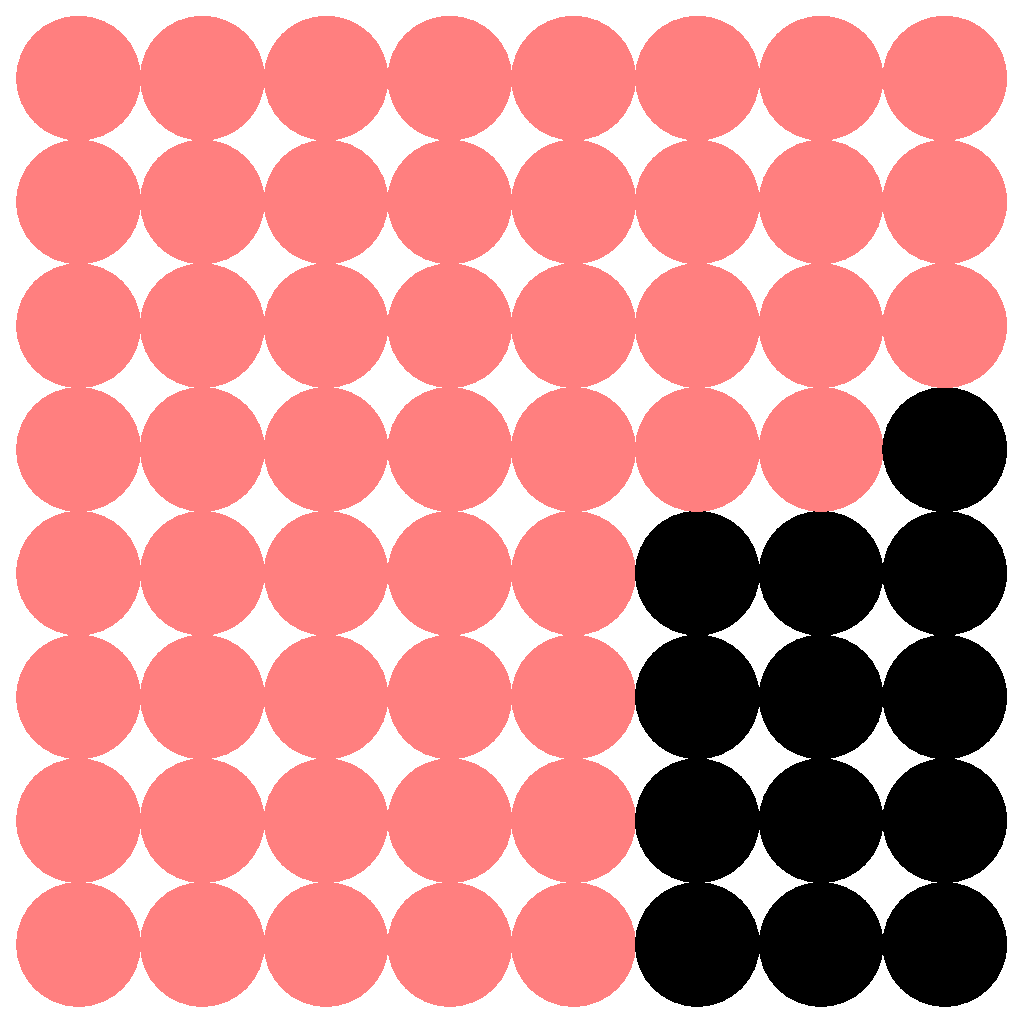
\includegraphics[scale=0.25]{s_f_do1.ps}
\hfill\ \\
{\bf a.} Construction of a partition with $13$ vertices (in black)
on a $8\times 8$ bidimensional mesh architecture.
}\ \hfill\
\parbox[t]{5.8cm}{
\hfill
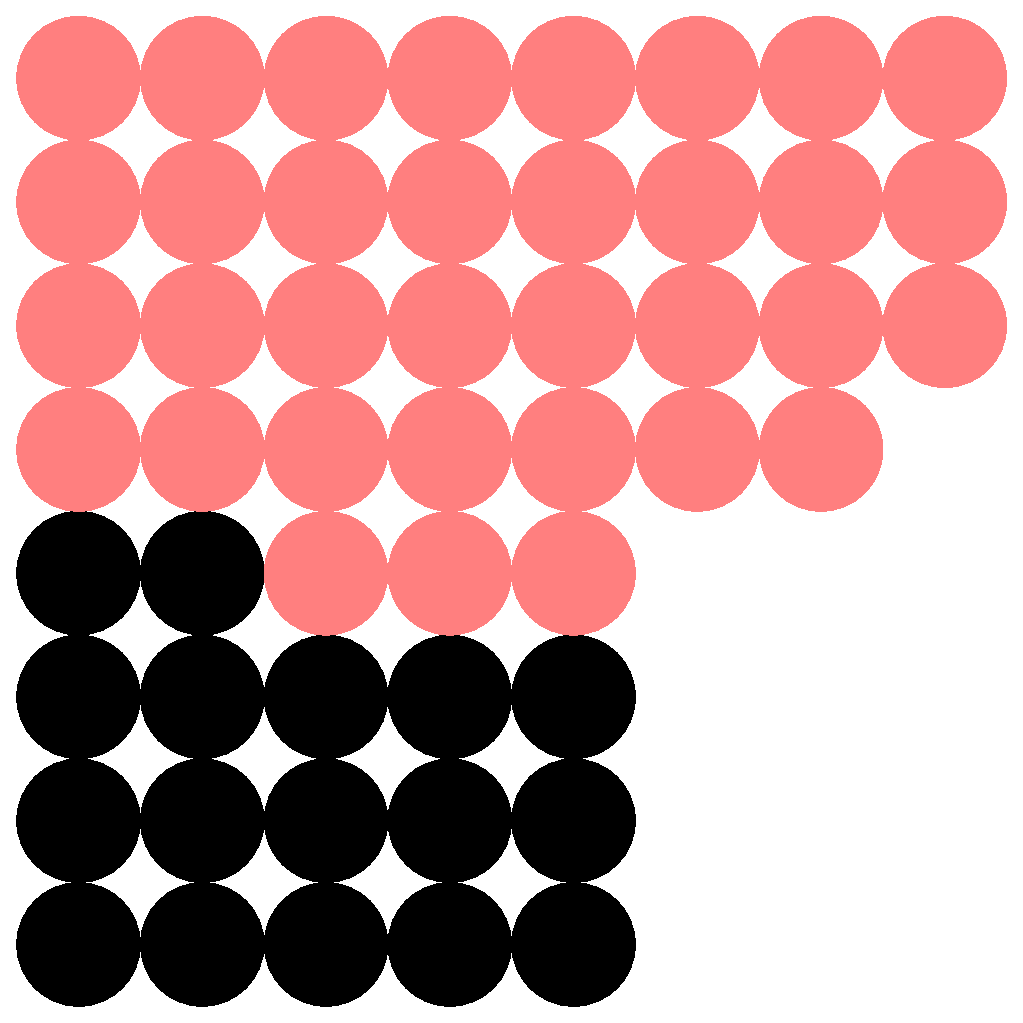
\includegraphics[scale=0.25]{s_f_do2.ps}
\hfill\ \\
{\bf b.} Construction of a partition with $17$ vertices (in black)
on the remaining architecture.
}\hfill\
\caption%
{Construction of partitions on a bidimensional $8\times 8$ mesh architecture
 by weighted bipartitioning.}
\label{fig-biparch}
\end{figure}

\progopt
\begin{itemize}
\iteme[\texttt{-h}]
Display the program synopsis.
\iteme[\texttt{-m}{\it method}]
Select the bipartitioning method (for \texttt{amk\_m2} only).
\begin{itemize}
\iteme[\texttt{n}]
Nested dissection.
\iteme[\texttt{o}]
Dimension-per-dimension one-way dissection. This is less efficient
than nested dissection, and this feature exists only for benchmarking
purposes.
\iteme[\texttt{-V}]
Print the program version and copyright.
\end{itemize}
\end{itemize}
\end{itemize}

\subsubsection{\texttt{amk\_grf}}
\label{sec-prog-amkgrf}

\begin{itemize}
\progsyn
\texttt{amk\_grf} [{\it input\_graph\_file} [{\it output\_target\_file}]] {\it options}

\progdes
The program \texttt{amk\_grf} turns a source graph file into a
decomposition-defined target architecture file.

The \texttt{-2} option creates a ``\texttt{deco~2}'' decomposition
rather than a ``\texttt{deco~0}'' one. See
Section~\ref{sec-file-target-deco},
page~\pageref{sec-file-target-deco} for more information on the
different types of decomposition-defined target architectures.

The \texttt{-l} option restricts the target architecture to the vertices indicated
in the given vertex list file. It is therefore possible
to build a target architecture made of several disconnected parts of a bigger
architecture.
Note that this is not equivalent to turning a disconnected source graph into
a target architecture, since doing so would lead to an architecture made of
several independent pieces at infinite distance one from another.
Considering the selected vertices within their original architecture makes
it possible to compute the distance between vertices belonging to distinct
connected components, and therefore to evaluate the cost of the mapping of
two neighbor processes onto disjoint areas of the architecture.
\\
The restriction feature is very useful in the context of multi-user parallel
machines. On these machines, when users request processors in order to run
their jobs, the partitions allocated by the operating system may not be
regular nor connected, because of existing partitions already attributed
to other people.
By feeding \texttt{amk\_grf} with the source graph representing the
whole parallel machine, and the vertex list containing the labels of the
processors allocated by the operating system, it is possible to build a
target architecture corresponding to this partition, and therefore to map
processes on it, automatically, regardless of the partition shape.

The \texttt{-b} option selects the recursive bipartitioning strategy used
to build the ``\texttt{deco~0}'' decomposition of the source
graph. For regular, unweighted, topologies, the \texttt{'-b(g|h)fx'}
recursive bipartitioning strategy should work best. For irregular or
weighted graphs, use the default strategy, which is more flexible. See
also the manual page of function \texttt{SCOTCH\_\lbt arch\lbo Build0},
page~\pageref{sec-lib-arch-build}, for further information.

\progopt
\begin{itemize}
\iteme[\texttt{-b}{\it strategy}]
Use recursive bipartitioning strategy {\it strategy\/} to build the
decomposition of the architecture graph. The format of bipartitioning
strategies is defined within section~\ref{sec-lib-format-map},
at page~\pageref{sec-lib-format-bipart}.
\iteme[\texttt{-h}]
Display the program synopsis.
\iteme[\texttt{-l}{\it input\_vertex\_file}]
Load vertex list from {\it input\_vertex\_file}. As for all other file names,
``\texttt{-}'' may be used to indicate standard input.
\iteme[\texttt{-V}]
Print the program version and copyright.
\end{itemize}
\end{itemize}

\subsubsection{\texttt{atst}}

\begin{itemize}
\progsyn
\texttt{atst} [{\it input\_target\_file} [{\it output\_data\_file}]] {\it options}

\progdes
The program \texttt{atst} is the architecture tester. It gives some statistics on
decomposition-defined target architectures, and in particular the
minimum, maximum, and average communication costs (that is, weighted distance)
between all pairs of processors.

\progopt
\begin{itemize}
\iteme[\texttt{-h}]
Display the program synopsis.
\iteme[\texttt{-V}]
Print the program version and copyright.
\end{itemize}
\end{itemize}

\subsubsection{\texttt{gcv}}
\label{sec-prog-gcv}

\begin{itemize}
\progsyn
\texttt{gcv} [{\it input\_graph\_file} [{\it output\_graph\_file} [{\it output\_geometry\_file}]]] {\it options}

\progdes
The program \texttt{gcv} is the source graph converter. It takes on input a graph
file of the format specified with the \texttt{-i} option, and outputs its
equivalent in the format specified with the \texttt{-o} option, along with its
associated geometry file whenever geometry data is available.
At the time being, it accepts four input formats: the Matrix Market
format~\cite{bopore96}, the Harwell-Boeing collection
format~\cite{dugrle92}, the \textsc{Chaco}/\metis\ graph
format~\cite{hele93c}, and the \scotch\ format.  Three output format
are available: the Matrix Market format, the {\sc Chaco}/\metis\ graph
format and the \scotch\ source graph and geometry data format.
\progopt
\begin{itemize}
\iteme[\texttt{-h}]
Display the program synopsis.
\iteme[\texttt{-i}{\it format}]
Specify the type of input graph.
The available input formats are listed below.
\begin{itemize}
\iteme[{\texttt{b}[{\it number}]}]
Harwell-Boeing graph collection format. Only symmetric assembled matrices
are currently supported.
Since files in this format can contain several graphs one after another,
the optional integer {\it number}, starting
from $0$, indicates which graph of the file is considered for conversion.
\iteme[\texttt{c}]
{\sc Chaco v1.0}/\metis\ format.
\iteme[\texttt{m}]
The Matrix Market format.
\iteme[\texttt{s}]
\scotch\ source graph format.
%% \iteme[\texttt{u}]
%% Universal Data Set 2412 format. On output, this node/element structure is
%% turned into a communication graph such that vertices represent elements and
%% there exists an edge between two vertices if the two end elements share a node
%% in the original UDS graph.
%% Since UDS format files are tag files, they do not have a well defined end.
%% Therefore, one cannot append data of different nature to the input stream
%% used to read this graph, since it will make the graph loading routine fail.
\end{itemize}
\iteme[\texttt{-o}{\it format}]
Specify the output graph format. The available output formats are listed below.
\begin{itemize}
\iteme[\texttt{c}]
{\sc Chaco v1.0}/\metis\ format.
\iteme[\texttt{m}]
The Matrix Market format.
\iteme[\texttt{s}]
\scotch\ source graph format.
\end{itemize}
\iteme[\texttt{-V}]
Print the program version and copyright.
\end{itemize}

Default option set is ``\texttt{-Ib0 -Os}''.
\end{itemize}

\subsubsection{\texttt{gmap} / \texttt{gpart}}
\label{sec-prog-gmap}

\begin{itemize}
\progsyn
\texttt{gmap} [{\it input\_graph\_file} [{\it input\_target\_file} [{\it output\_mapping\_file} [{\it output\_log\_file}]]]] {\it options}\\
~\\
\texttt{gpart} {\it number\_\lbt of\_\lbt parts} [{\it input\_graph\_file} [{\it output\_mapping\_file} [{\it output\_log\_file}]]] {\it options}

\progdes
The program \texttt{gmap} is the graph mapper. It uses a partitioning
strategy to map a source graph onto a target graph, so that the weight of
source graph vertices allocated to target vertices is balanced, and the
communication cost function $f_C$ is minimized.

The program \texttt{gpart} is the graph partitioner. It uses a
partitioning strategy to split a source graph into the prescribed
number of parts, using vertex or edge separators, depending whether
the \texttt{-o} option is set or not.

The implemented mapping methods mainly derive from graph theory.  In
particular, graph geometry is never used, even if it is available;
only topological properties are taken into account. Mapping methods
are used to define mapping strategies by means of selection,
combination, grouping, and condition operators.
\\

Mapping methods implemented in version~{\sc 6.0} comprise direct k-way
methods, including a k-way multilevel framework and k-way local
refinement methods, as well as the Dual
Recursive Bipartitioning algorithm, which uses graph bipartitioning
methods. Available bipartitioning methods include a multilevel
framework that uses other bipartitioning methods to compute the
initial and refined bipartitions: an improved implementation of the
Fiduccia--Mattheyses heuristic designed to handle weighted graphs,
a diffusion-based algorithm, a greedy method derived from the Gibbs,
Poole, and Stockmeyer algorithm, a greedy graph growing heuristic, a
greedy ``exactifying'' refinement algorithm designed to balance vertex
loads as much as possible, etc.

\texttt{gpart} is a simplified interface to \texttt{gmap}, which performs
graph partitioning instead of static mapping. Consequently, the
desired number of parts has to be provided, in lieu of the target
architecture.

The \texttt{-b} and \texttt{-c} options allow the user to set preferences on
the behavior of the mapping strategy which is used by default. The
\texttt{-m} option allows the user to define a custom mapping strategy.

Both programs can be used to perform clustering, by means of the
\texttt{-q} option. \texttt{gpart} will perform topology-independent
clustering, while \texttt{gmap} may compute locality-preserving clusters
when mapping onto variable-sized, non-complete, architectures (see
Section~\ref{sec-file-target-variable}).

If mapping statistics are wanted rather than the mapping output itself,
mapping output can be set to \texttt{/dev/null}, with option \texttt{-vmt}
to get mapping statistics and timings.

\progopt\\*
Since the program is devoted to experimental studies, it has many
optional parameters, used to test various execution modes. Values
set by default will give best results in most cases.
\begin{itemize}
\iteme[\texttt{-b}{\it rat}]
Set the maximum load imbalance ratio to \textit{rat}, which should
be a value comprised between $0$ and $1$. This option can be used in
conjunction with option \texttt{-c}, but is incompatible with option
\texttt{-m}.
\iteme[\texttt{-c}{\it flags}]
Tune the default mapping strategy according to the given preference
flags. Some of these flags are antagonistic, while others can be
combined. See Section~\ref{sec-lib-format-strat-default} for more
information. The currently available flags are the following.
\begin{itemize}
\iteme[\texttt{b}]
Enforce load balance as much as possible.
\iteme[\texttt{q}]
Privilege quality over speed.
\iteme[\texttt{r}]
Only use recursive bipartitioning methods.
\iteme[\texttt{s}]
Privilege speed over quality.
\iteme[\texttt{t}]
Use only safe methods in the strategy.
\end{itemize}
This option can be used in conjunction with option \texttt{-b}, but is
incompatible with option \texttt{-m}.
The resulting strategy string can be displayed by means
of the \texttt{-vs} option.
\iteme[\texttt{-h}]
Display the program synopsis.
\iteme[\texttt{-m}{\it strat\/}]
Apply mapping strategy {\it strat}. In the case of static mapping or
of edge-based graph partitioning, the format of mapping strategies
should comply with the format defined in
Section~\ref{sec-lib-format-map}.  If the \texttt{-o} option is used (see
below), strategies must be vertex partitioning strategies, which are
described in Section~\ref{sec-lib-format-part-ovl}.
This option is incompatible with options \texttt{-b} and
\texttt{-c}.
\iteme[\texttt{-o}]
Compute vertex-based partitions rather than static mappings or
edge-based partitions. This option is only valid for \texttt{gpart}, or
when \texttt{gmap} is called with a target architecture which is an
unweighted complete graph.
\iteme[\texttt{-q}] (for \texttt{gpart})
\iteme[\texttt{-q}{\it pwght}] (for \texttt{gmap})
Perform clustering instead of partitioning or mapping. Clustering is
achieved by means of a specific strategy string that performs
recursive bipartitioning until the size of the parts is smaller than
some threshold value. For \texttt{gpart}, this value replaces the desired
number of parts as the first argument passed to the program. For
\texttt{gmap}, the threshold must be given just after the \texttt{-q} option.
\iteme[\texttt{-s}{\it obj}]
Mask source edge and vertex weights. This option allows the user to
``unweight'' weighted source graphs by removing weights from edges and
vertices at loading time. {\it obj\/} may contain several of the following
switches.
\begin{itemize}
\iteme[\texttt{e}]
Remove edge weights, if any.
\iteme[\texttt{v}]
Remove vertex weights, if any.
\end{itemize}
\iteme[\texttt{-V}]
Print the program version and copyright.
\iteme[\texttt{-v}{\it verb}]
Set verbose mode to {\it verb}, which may contain several of the following
switches. For a detailed description of the data displayed, please
refer to the manual page of \texttt{gmtst} below.
\begin{itemize}
\iteme[\texttt{m}]
Mapping or partitioning information, depending whether the \texttt{-o}
option has been set or not.
\iteme[\texttt{s}]
Strategy information. This parameter displays the mapping
strategy which will be used by \texttt{gmap} or \texttt{gpart}.
\iteme[\texttt{t}]
Timing information.
\end{itemize}
\iteme[\texttt{-V}]
Print the program version and copyright.
\end{itemize}
\end{itemize}

\subsubsection{\texttt{gmk\_}*}

\begin{itemize}
\progsyn
\texttt{gmk\_hy} {\it dim} [{\it output\_graph\_file}] {\it options}\\
~\\
\texttt{gmk\_m2} {\it dimX} [{\it dimY} [{\it output\_graph\_file}]] {\it options}\\
~\\
\texttt{gmk\_m3} {\it dimX} [{\it dimY} [{\it dimZ} [{\it output\_graph\_file}]]] {\it options}\\
~\\
\texttt{gmk\_ub2} {\it dim} [{\it output\_graph\_file}] {\it options}

\progdes
The \texttt{gmk\_}* programs make source graphs.
Each of them is devoted to a specific topology, for which it builds target
graphs of any dimension.
\\
The \texttt{gmk\_}* programs are mainly used in conjunction with \texttt{amk\_grf}.
Most \texttt{gmk\_}* programs build source graphs
describing parallel machines, which are used by \texttt{amk\_grf} to generate
corresponding target sub-architectures, by means of its \texttt{-l}
option.
Such a procedure is shown in section~\ref{sec-examples}, which builds a target
architecture from five vertices of a binary de~Bruijn graph of dimension~$3$.
\\

\noi
Program \texttt{gmk\_hy} outputs the source file of a hypercube graph of
dimension {\it dim}. Vertices are labeled according to the decimal value
of their binary representation.
\\

\noi
Program \texttt{gmk\_m2} outputs the source file of a bidimensional mesh
with {\it dimX\/} columns and {\it dimY\/} rows. If the \texttt{-t}
option is set, tori are built instead of meshes. The vertex of
coordinates $(\mbox{\it posX},\mbox{\it posY\/})$ is labeled
$\mbox{\it posY} \times \mbox{\it dimX} + \mbox{\it posX}$.
\\

\noi
Program \texttt{gmk\_m3} outputs the source file of a tridimensional mesh
with {\it dimZ} layers of {\it dimY\/} rows by {\it dimX\/}
columns. If the \texttt{-t} option is set, tori are built instead of
meshes. The vertex of coordinates $(\mbox{\it posX},\mbox{\it
posY\/})$ is labeled $(\mbox{\it posZ} \times \mbox{\it dimY} +
\mbox{\it posY}) \times \mbox{\it dimX} + \mbox{\it posX}$.
\\

\noi
Program \texttt{gmk\_ub2} outputs the source file of a binary unoriented
de~Bruijn graph of dimension {\it dim}. Vertices are labeled according to
the decimal value of their binary representation.

\progopt
\begin{itemize}
\iteme[\texttt{-g}{\it output\_geometry\_file}]
Output graph geometry to file {\it output\_geometry\_file}
(for \texttt{gmk\_m2} only).
As for all other file names, ``\texttt{-}''
may be used to indicate standard output.
\iteme[\texttt{-h}]
Display the program synopsis.
\iteme[\texttt{-t}]
Build a torus rather than a mesh (for \texttt{gmk\_m2} only).
\iteme[\texttt{-V}]
Print the program version and copyright.
\end{itemize}
\end{itemize}

\subsubsection{\texttt{gmk\_msh}}
\label{sec-prog-gmkmsh}

\begin{itemize}
\progsyn
\texttt{gmk\_msh} [{\it input\_mesh\_file} [{\it output\_graph\_file}]] {\it options}\\

\progdes
The \texttt{gmk\_msh} program builds a graph file from a mesh file. All
of the nodes of the mesh are turned into graph vertices, and edges
are created between all pairs of vertices that share an element (that
is, elements are turned into cliques).

\progopt
\begin{itemize}
\iteme[\texttt{-h}]
Display the program synopsis.
\iteme[\texttt{-V}]
Print the program version and copyright.
\end{itemize}
\end{itemize}

\subsubsection{\texttt{gmtst}}

\begin{itemize}
\progsyn
\texttt{gmtst} [{\it input\_graph\_file} [{\it input\_\lbt target\_\lbt file} [{\it input\_\lbt mapping\_\lbt file} [{\it output\_\lbt data\_\lbt file}]]]] {\it options}

\progdes
The program \texttt{gmtst} is the graph mapping tester. It outputs some
statistics on the given mapping, regarding load balance and inter-processor
communication.
\\
The two first statistics lines deal with process mapping statistics, while
the following ones deal with communication statistics.
The first mapping line gives the number of processors used by
the mapping, followed by the number of processors available in the
architecture, and the ratio of these two numbers, written between parentheses.
The second mapping line gives the minimum, maximum, and average loads of the
processors, followed by the variance of the load distribution, and an imbalance
ratio equal to the maximum load over the average load.
The first communication line gives the minimum and maximum number of neighbors
over all blocks of the mapping, followed by the sum of the number of neighbors
over all blocks of the mapping, that is the total number of messages
that have to be sent to exchange data between all neighboring blocks.
The second communication line gives the average dilation of the edges,
followed by the sum of all edge dilations.
The third communication line gives the average expansion of the edges,
followed by the value of function $f_C$.
The fourth communication line gives the average cut of the edges,
followed by the number of cut edges.
The fifth communication line shows the ratio of the average expansion over
the average dilation; it is smaller than $1$ when the mapper succeeds in
putting heavily intercommunicating processes closer to each other than it
does for lightly communicating processes; it is equal to $1$ if all edges
have the same weight.
The remaining lines form a distance histogram, which shows the amount of
communication load that involves processors located at increasing distances.

\texttt{gmtst} allows the testing of cross-architecture mappings. By inputing it
a target architecture different from the one that has been used to compute the
mapping, but with compatible vertex labels, one can see what the mapping
would yield on this new target architecture.

\progopt
\begin{itemize}
\iteme[\texttt{-h}]
Display the program synopsis.
\iteme[\texttt{-V}]
Print the program version and copyright.
\end{itemize}
\end{itemize}

\subsubsection{\texttt{gord}}

\begin{itemize}
\progsyn
\texttt{gord} [{\it input\_graph\_file} [{\it output\_ordering\_file} [{\it output\_log\_file}]]] {\it options}

\progdes
The \texttt{gord} program is the block sparse matrix graph orderer. It uses an
ordering strategy to compute block orderings of sparse matrices
represented as source graphs, whose vertex weights indicate the number
of DOFs per node (if this number is non homogeneous) and whose edges
are unweighted, in order to minimize fill-in and operation count.

Since its main purpose is to provide orderings that exhibit high
concurrency for parallel block factorization, it comprises a nested
dissection method~\cite{geli81}, but classical~\cite{liu-85} and
state-of-the-art~\cite{amdadu96,peroam99} minimum degree algorithms
are implemented as well.
Ordering methods are used to define ordering strategies by means of
selection, grouping, and condition operators.

For the nested dissection method, vertex separation methods comprise
algorithms that directly compute vertex separators, as well as methods
that build vertex separators from edge separators, \ie graph
bipartitions (all of the graph bipartitioning methods available in the
static mapper \texttt{gmap} can be used in this latter case).

The \texttt{-o} option allows the user to define the ordering
strategy. The \texttt{-c} option allows the user to set preferences on
the behavior of the ordering strategy which is used by default.
\\

When the graphs to order are very large, the same results can
be obtained by using the \texttt{dgord} parallel program of the
\ptscotch\ distribution, which can read centralized graph
files too.

\progopt\\*
Since the program is devoted to experimental studies, it has many
optional parameters, used to test various execution modes. Values
set by default will give best results in most cases.
\begin{itemize}
\iteme[\texttt{-c}{\it flags}]
Tune the default ordering strategy according to the given preference
flags. Some of these flags are antagonistic, while others can be
combined. See Section~\ref{sec-lib-format-strat-default} for more
information. The resulting strategy string can be displayed by means
of the \texttt{-vs} option.
\begin{itemize}
\iteme[\texttt{b}]
Enforce load balance as much as possible.
\iteme[\texttt{q}]
Privilege quality over speed. This is the default behavior.
\iteme[\texttt{s}]
Privilege speed over quality.
\iteme[\texttt{t}]
Use only safe methods in the strategy.
\end{itemize}
\iteme[\texttt{-h}]
Display the program synopsis.
\iteme[\texttt{-m}{\it output\_mapping\_file}]
Write to {\it output\_mapping\_file\/} the mapping of graph vertices to
column blocks. All of the separators and leaves produced by the nested
dissection method are considered as distinct column blocks, which may
be in turn split by the ordering methods that are applied to them.
Distinct integer numbers are associated with each of the column blocks,
such that the number of a block is always greater than the ones of its
predecessors in the elimination process, that is, its descendants in the
elimination tree.
The structure of mapping files is given in section~\ref{sec-file-map}.

When the geometry of the graph is available, this mapping file may be
processed by program \texttt{gout} to display the vertex separators and
supervariable amalgamations that have been computed.
\iteme[{\texttt{-o}{\it strat}}]
Apply ordering strategy {\it strat}. The format of ordering
strategies is defined in section~\ref{sec-lib-format-ord}.
\iteme[\texttt{-t}{\it output\_tree\_file}]
Write to {\it output\_tree\_file\/} the structure of the separator
tree. The data that is written resembles much the one of a mapping
file: after a first line that contains the number of lines to follow,
there are that many lines of mapping pairs, which associate an integer
number with every graph vertex index. This integer number is the
number of the column block which is the parent of the column block to
which the vertex belongs, or $-1$ if the column block to which the
vertex belongs is a root of the separator tree (there can be several
roots, if the graph is disconnected).

Combined to the column block mapping data produced by option \texttt{-m},
the tree structure allows one to rebuild the separator tree.
\iteme[\texttt{-V}]
Print the program version and copyright.
\iteme[\texttt{-v}{\it verb}]
Set verbose mode to {\it verb}, which may contain several of the following
switches.
%For a detailed description of the data displayed, please
%refer to the manual page of \texttt{gotst}.
\begin{itemize}
\iteme[\texttt{s}]
Strategy information. This parameter displays the ordering
strategy which will be used by \texttt{gord}.
\iteme[\texttt{t}]
Timing information.
\end{itemize}
\end{itemize}
\end{itemize}

\subsubsection{\texttt{gotst}}
\label{sec-prog-gotst}

\begin{itemize}
\progsyn
\texttt{gotst} [{\it input\_graph\_file} [{\it input\_ordering\_file} [{\it output\_data\_file}]]] {\it options}

\progdes
The program \texttt{gotst} is the ordering tester. It gives some
statistics on orderings, including the number of non-zeros and
the operation count of the factored matrix, as well as statistics
regarding the elimination tree. Since it performs the factorization
of the reordered matrix, it can take a very long time and consume
a large amount of memory when applied to large graphs.
\\
The first two statistics lines deal with the elimination tree. The
first one displays the number of leaves, while the second shows
the minimum height of the tree (that is, the
length of the shortest path from any leaf to the --or a-- root node),
its maximum height, its average height, and the variance of the
heights with respect to the average.
The third line displays the number of non-zero terms in the factored
matrix, the amount of index data that is necessary to maintain the
block structure of the factored matrix, and the number of operations
required to factor the matrix by means of Cholesky factorization.

\progopt
\begin{itemize}
\iteme[\texttt{-h}]
Display the program synopsis.
\iteme[\texttt{-v}]
Do not account for vertex weights when computing factorization costs.
\iteme[\texttt{-V}]
Print the program version and copyright.
\end{itemize}
\end{itemize}

\subsubsection{\texttt{gout}}
\label{sec-prog-gout}

\begin{itemize}
\progsyn
\texttt{gout} [{\it input\_graph\_file} [{\it input\_geometry\_file} [{\it input\_\lbt mapping\_\lbt file} [{\it output\_\lbt visualization\_\lbt file}]]]] {\it options}

\progdes
The \texttt{gout} program is the graph, matrix, and mapping viewer program. It
takes on input a source graph, its geometry file, and optionally a mapping
result file, and produces a file suitable for display.
At the time being, \texttt{gout} can generate plain and encapsulated PostScript
files for the display of adjacency matrix patterns and the
display of planar graphs (although tridimensional objects
can be displayed by means of isometric projection, the display of
tridimensional mappings is not efficient), and {\sc Open Inventor}
files~\cite{oinv} for the interactive visualization of
tridimensional graphs.
\\
In the case of mapping display,
the number of mapping pairs contained in the input mapping file may
differ from the number of vertices of the input source graph;
only mapping pairs the source labels of which match labels of source graph
vertices will be taken into account for display.
This feature allows the user to show the result of the mapping of a subgraph
drawn on the whole graph, or else to outline the most important aspects
of a mapping by restricting the display to a limited portion of the graph.
For example, Figure~\ref{fig-out-ps}\@.b shows how the result of the mapping of
a subgraph of the bidimensional mesh $\MD(4,4)$ onto the complete graph
$\KP(2)$ can be displayed on the whole $\MD(4,4)$ graph,
and Figure~\ref{fig-out-ps}\@.c shows how the display of the same mapping
can be restricted to a subgraph of the original graph.
% gmk_m2 4 4 s_f_out1.grf -gs_f_out.xyz
% map s_f_out2.grf ../tgt/k2.tgt s_f_out2.map
% out s_f_out2.grf s_f_out.xyz -m - s_f_out1.ps '-Op{e,g,l}'
% out s_f_out1.grf s_f_out.xyz s_f_out2.map s_f_out2.ps '-Op{e,g,l}'
% out s_f_out3.grf s_f_out.xyz s_f_out2.map s_f_out3.ps '-Op{e,g,l}'
\begin{figure}[hbt]
\hfill
\parbox[t]{4.5cm}{
\hfill
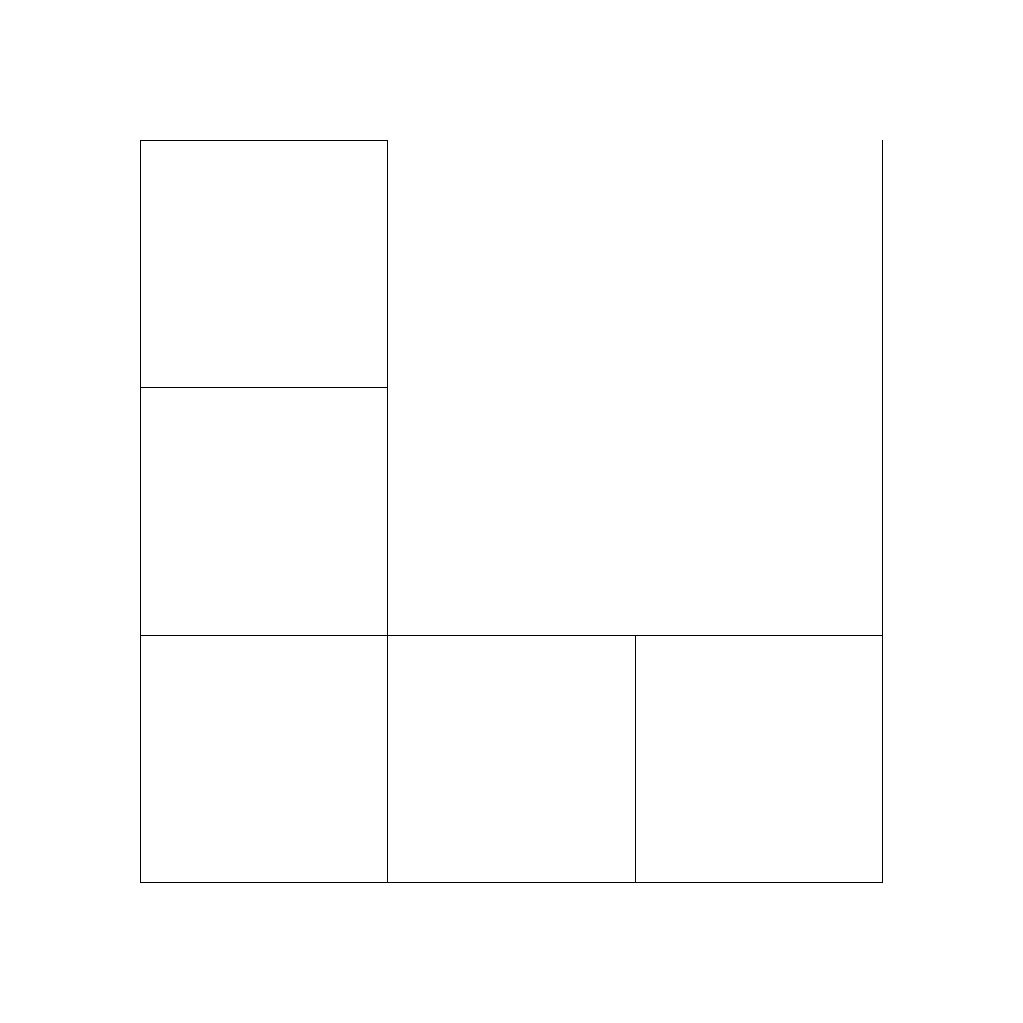
\includegraphics[scale=0.25]{s_f_out1.ps}
\hfill\ \\
{\bf a.} A subgraph of $\MD(4,4)$ to be mapped onto $\KP(2)$.
}\ \hfill\
\parbox[t]{4.5cm}{
\hfill
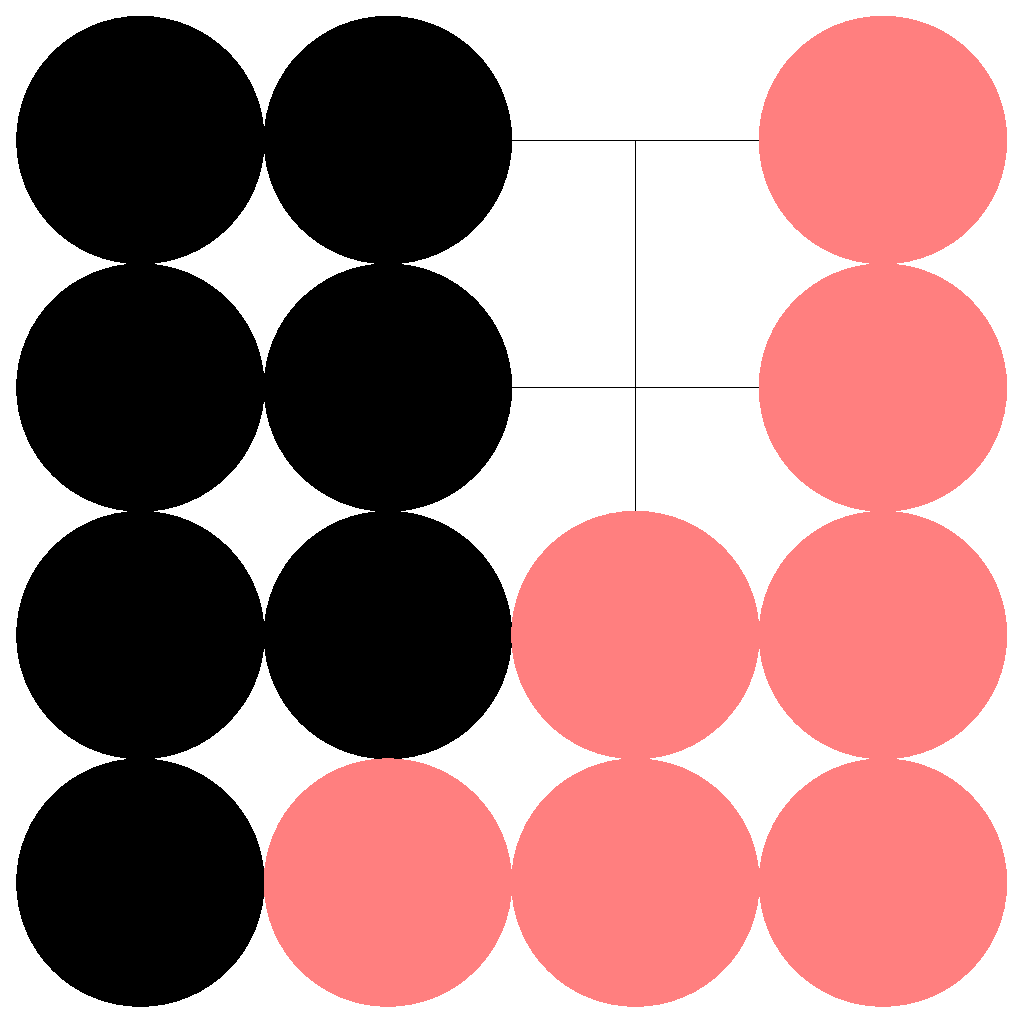
\includegraphics[scale=0.25]{s_f_out2.ps}
\hfill\ \\
{\bf b.} Mapping result displayed on the full $\MD(4,4)$ graph.
}\ \hfill\
\parbox[t]{4.5cm}{
\hfill
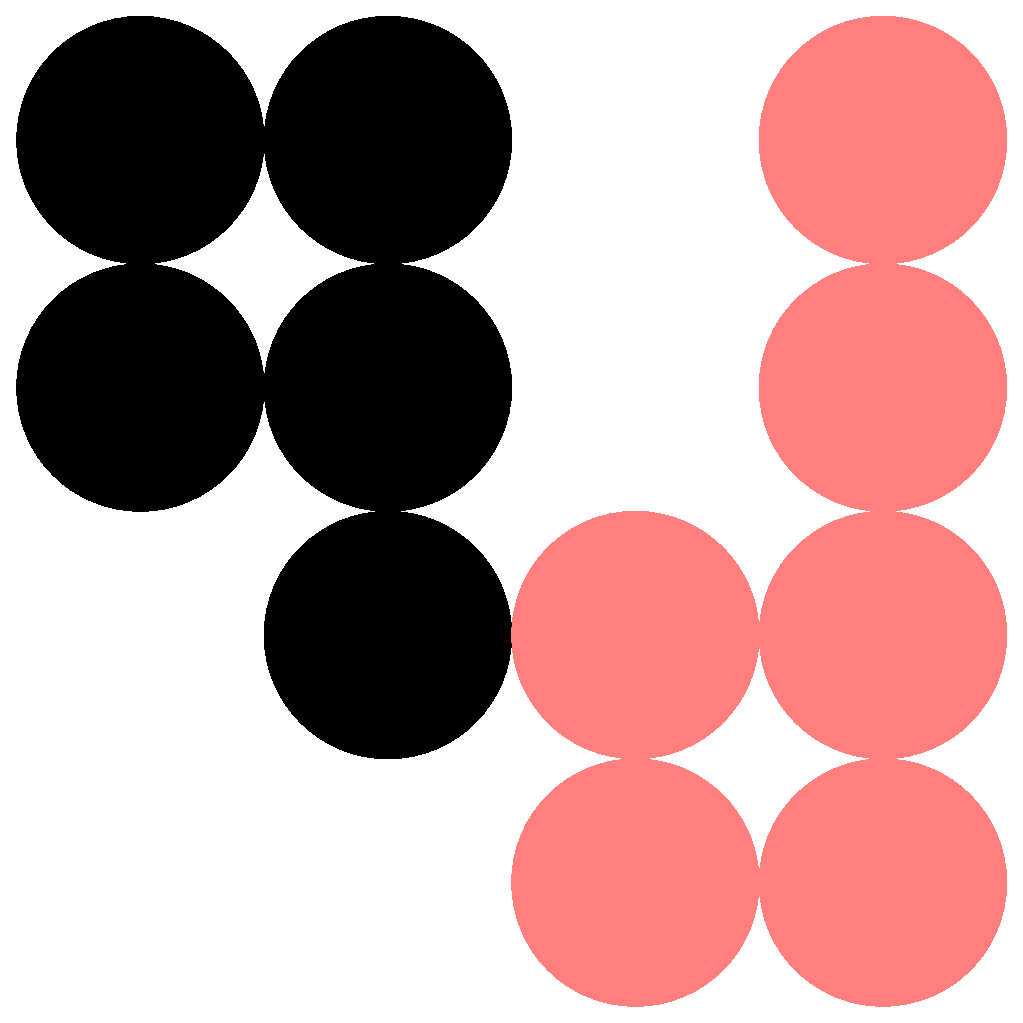
\includegraphics[scale=0.25]{s_f_out3.ps}
\hfill\ \\
{\bf c.} Mapping result displayed on another subgraph of $\MD(4,4)$.
}\hfill\
\caption{PostScript diplay of a single mapping file with different
         subgraphs of the same source graph. Vertices covered with disks
         of the same color are mapped onto the same processor.}
\label{fig-out-ps}
\end{figure}

\progopt
\begin{itemize}
\iteme[\texttt{-g}{\it parameters}]
Geometry parameters.
\begin{itemize}
\iteme[\texttt{n}]
Do not read geometry data. This option can be used in conjunction with
option \texttt{-om} to avoid reading the geometry file when displaying
the pattern of the adjacency matrix associated with the source graph,
since geometry data are not needed in this case.
If this option is set, the geometry file is not read. However, if an
{\it output\_\lbt visualization\_\lbt file} name is given in the
command line, dummy {\it input\_\lbt geometry\_\lbt file\/} and {\it
input\_\lbt mapping\_\lbt file\/} names must be specified so that the
file argument count is correct. In this case, use the ``\texttt{-}''
parameter to take standard input as a dummy geometry input stream.  In
practice, the \texttt{-om} and \texttt{-gn} options always imply the
\texttt{-mn} option.
\iteme[\texttt{r}]
For bidimensional geometry only, rotate geometry data by $90$ degrees,
counter-clockwise.
\end{itemize}
\iteme[\texttt{-h}]
Display the program synopsis.
\iteme[\texttt{-mn}]
Do not read mapping data, and display the graph without any mapping
information. If this option is set, the mapping file is not
read. However, if an {\it output\_\lbt visualization\_\lbt file\/}
name is given in the command line, a dummy {\it input\_\lbt
mapping\_\lbt file\/} name must be specified so that the file argument
count is correct. In this case, use the ``\texttt{-}'' parameter to take
standard input as a dummy mapping input stream.
\iteme[{\texttt{-o}{\it format}[\texttt{\{}{\it parameters}\texttt{\}}]}]
Specify the type of output, with optional parameters within curly braces
and separated by commas. The output formats are listed below.
\begin{itemize}
\iteme[\texttt{i}]
Output the graph in SGI's {\sc Open Inventor} format, in ASCII mode,
suitable for display by the \texttt{ivview} program~\cite{oinv}. The
optional parameters are given below.
\begin{itemize}
\iteme[\texttt{c}]
Color output, using $16$ different colors. Opposite of \texttt{g}.
\iteme[\texttt{g}]
Grey-level output, using $8$ different levels. Opposite of \texttt{c}.
\iteme[\texttt{r}]
Remove cut edges. Edges the ends of which are mapped onto different
processors are not displayed. Opposite of \texttt{v}.
\iteme[\texttt{v}]
View cut edges. All graph edges are displayed.
Opposite of \texttt{r}.
\end{itemize}
\iteme[\texttt{m}]
Output the pattern of the adjacency matrix associated with the source graph,
in Adobe's PostScript format. The optional parameters are given below.
\begin{itemize}
\iteme[\texttt{e}]
Encapsulated PostScript output, suitable for \LaTeX\ use with \texttt{epsf}.
Opposite of \texttt{f}.
\iteme[\texttt{f}]
Full-page PostScript output, suitable for direct printing.
Opposite of \texttt{e}.
\end{itemize}
\iteme[\texttt{p}]
Output the graph in Adobe's PostScript format.
The optional parameters are given below.
\begin{itemize}
\iteme[\texttt{a}]
Avoid displaying the mapping disks. Opposite of \texttt{d}.
\iteme[\texttt{c}]
Color PostScript output, using $16$ different colors. Opposite of \texttt{g}.
\iteme[\texttt{d}]
Display the mapping disks. Opposite of \texttt{a}.
\iteme[\texttt{e}]
Encapsulated PostScript output, suitable for \LaTeX\ use with \texttt{epsf}.
Opposite of \texttt{f}.
\iteme[\texttt{f}]
Full-page PostScript output, suitable for direct printing.
Opposite of \texttt{e}.
\iteme[\texttt{g}]
Grey-level PostScript output. Opposite of \texttt{c}.
\iteme[\texttt{l}]
Large clipping. Mapping disks are included in the clipping area computation.
Opposite of \texttt{s}.
\iteme[\texttt{r}]
Remove cut edges. Edges the ends of which are mapped onto different
processors are not displayed.
Opposite of \texttt{v}.
\iteme[\texttt{s}]
Small clipping. Mapping disks are excluded from the clipping area computation.
Opposite of \texttt{l}.
\iteme[\texttt{v}]
View cut edges. All graph edges are displayed.
Opposite of \texttt{r}.
\iteme[\texttt{x=}{\it val}]
Minimum X relative clipping position (in [0.0;1.0]).
\iteme[\texttt{X=}{\it val}]
Maximum X relative clipping position (in [0.0;1.0]).
\iteme[\texttt{y=}{\it val}]
Minimum Y relative clipping position (in [0.0;1.0]).
\iteme[\texttt{Y=}{\it val}]
Maximum Y relative clipping position (in [0.0;1.0]).
\end{itemize}
\iteme[\texttt{v}]
Output the graph in VTK legacy ASCII format, suitable for display by
the \texttt{paraview} program~\cite{paraview}. The graph partition is
represented as an integer scalar dataset called \texttt{mapValues}.
Unmapped vertices are assigned to part index~\texttt{0}, while higher
part indices represent regular parts (hence, part number $i$ of some
mapping becomes part index $i+1$ in the VTK dataset).
The optional parameters are given below.
\begin{itemize}
\iteme[\texttt{r}]
Remove cut edges. Edges the ends of which are mapped onto different
processors are not displayed. Opposite of \texttt{v}.
\iteme[\texttt{v}]
View cut edges. All graph edges are displayed.
Opposite of \texttt{r}.
\end{itemize}
\end{itemize}
\iteme[\texttt{-V}]
Print the program version and copyright.
\end{itemize}

Default option set is ``\texttt{-Oi\{v\}}''.
\end{itemize}

\subsubsection{\texttt{gtst}}

\begin{itemize}
\progsyn
\texttt{gtst} [{\it input\_graph\_file} [{\it output\_data\_file}]] {\it options}

\progdes
The program \texttt{gtst} is the source graph tester. It checks the
consistency of the input source graph structure (matching of arcs,
number of vertices and edges, etc\@.), and gives some statistics
regarding edge weights, vertex weights, and vertex degrees.
\\

When the graphs to test are very large, the same results can
be obtained by using the \texttt{dgtst} parallel program of the
\ptscotch\ distribution, which can read centralized graph
files too.

\progopt
\begin{itemize}
\iteme[\texttt{-h}]
Display the program synopsis.
\iteme[\texttt{-V}]
Print the program version and copyright.
\end{itemize}
\end{itemize}

\subsubsection{\texttt{mcv}}
\label{sec-prog-mcv}

\begin{itemize}
\progsyn
\texttt{mcv} [{\it input\_mesh\_file} [{\it output\_mesh\_file} [{\it output\_geometry\_file}]]] {\it options}

\progdes
The program \texttt{mcv} is the source mesh converter. It takes on input a mesh
file of the format specified with the \texttt{-i} option, and outputs its
equivalent in the format specified with the \texttt{-o} option, along with its
associated geometry file whenever geometrical data is available.
At the time being, it only accepts one external input format: the
Harwell-Boeing format~\cite{dugrle92}, for square elemental matrices only.
The only output format to date is the \scotch\ source mesh and
geometry data format.

\progopt
\begin{itemize}
\iteme[\texttt{-h}]
Display the program synopsis.
\iteme[\texttt{-i}{\it format}]
Specify the type of input mesh.
The available input formats are listed below.
\begin{itemize}
\iteme[{\texttt{b}[{\it number}]}]
Harwell-Boeing mesh collection format. Only symmetric elemental matrices
are currently supported.
Since files in this format can contain several meshes one after another,
the optional integer {\it number}, starting
from $0$, indicates which mesh of the file is considered for conversion.
\iteme[\texttt{s}]
\scotch\ source mesh format.
\end{itemize}
\iteme[\texttt{-o}{\it format}]
Specify the output graph format. The available output formats are listed below.
\begin{itemize}
\iteme[\texttt{s}]
\scotch\ source graph format.
\end{itemize}
\iteme[\texttt{-V}]
Print the program version and copyright.
\end{itemize}

Default option set is ``\texttt{-Ib0 -Os}''.
\end{itemize}

\subsubsection{\texttt{mmk\_}*}

\begin{itemize}
\progsyn
\texttt{mmk\_m2} {\it dimX} [{\it dimY} [{\it output\_mesh\_file}]] {\it options}\\
~\\
\texttt{mmk\_m3} {\it dimX} [{\it dimY} [{\it dimZ} [{\it output\_mesh\_file}]]] {\it options}\\

\progdes
The \texttt{mmk\_}* programs make source meshes.
\\

\noi
Program \texttt{mmk\_m2} outputs the source file of a bidimensional mesh
with $\mbox{{\it dimX\/}} \times \mbox{{\it dimY\/}}$ elements and
$(\mbox{{\it dimX\/}}+1) \times (\mbox{{\it dimY\/}}+1)$ nodes.
The element of coordinates $(\mbox{\it posX},\mbox{\it posY\/})$ is
labeled $\mbox{\it posY} \times \mbox{\it dimX} + \mbox{\it posX}$.
\\

\noi
Program \texttt{mmk\_m3} outputs the source file of a tridimensional mesh
with $\mbox{{\it dimX\/}} \times \mbox{{\it dimY\/}} \times
\mbox{{\it dimZ\/}}$ elements and $(\mbox{{\it dimX\/}}+1) \times
(\mbox{{\it dimY\/}}+1) \times (\mbox{{\it dimZ\/}}+1)$ nodes.
\\

\progopt
\begin{itemize}
\iteme[\texttt{-g}{\it output\_geometry\_file}]
Output mesh geometry to file {\it output\_geometry\_file}
(for \texttt{mmk\_m2} only).
As for all other file names, ``\texttt{-}''
may be used to indicate standard output.
\iteme[\texttt{-h}]
Display the program synopsis.
\iteme[\texttt{-V}]
Print the program version and copyright.
\end{itemize}
\end{itemize}

\subsubsection{\texttt{mord}}

\begin{itemize}
\progsyn
\texttt{mord} [{\it input\_mesh\_file} [{\it output\_ordering\_file} [{\it output\_log\_file}]]] {\it options}

\progdes
The \texttt{mord} program is the block sparse matrix mesh orderer. It
uses an ordering strategy to compute block orderings of sparse matrices
represented as source meshes, whose node vertex weights indicate the
number of DOFs per node (if this number is non homogeneous), in order
to minimize fill-in and operation count.

Since its main purpose is to provide orderings that exhibit high
concurrency for parallel block factorization, it comprises a nested
dissection method~\cite{geli81}, but classical~\cite{liu-85} and
state-of-the-art~\cite{amdadu96,peroam99} minimum degree algorithms
are implemented as well.
Ordering methods are used to define ordering strategies by means of
selection, grouping, and condition operators.

The \texttt{-o} option allows the user to define the ordering
strategy. The \texttt{-c} option allows the user to set preferences on
the behavior of the ordering strategy which is used by default.

\progopt\\*
Since the program is devoted to experimental studies, it has many
optional parameters, used to test various execution modes. Values
set by default will give best results in most cases.
\begin{itemize}
\iteme[\texttt{-c}{\it flags}]
Tune the default ordering strategy according to the given preference
flags. Some of these flags are antagonistic, while others can be
combined. See Section~\ref{sec-lib-format-strat-default} for more
information. The resulting strategy string can be displayed by means
of the \texttt{-vs} option.
\begin{itemize}
\iteme[\texttt{b}]
Enforce load balance as much as possible.
\iteme[\texttt{q}]
Privilege quality over speed. This is the default behavior.
\iteme[\texttt{s}]
Privilege speed over quality.
\iteme[\texttt{t}]
Use only safe methods in the strategy.
\end{itemize}
\iteme[\texttt{-h}]
Display the program synopsis.
\iteme[\texttt{-m}{\it output\_mapping\_file}]
Write to {\it output\_mapping\_file\/} the mapping of mesh node
vertices to column blocks. All of the separators and leaves produced
by the nested dissection method are considered as distinct column
blocks, which may be in turn split by the ordering methods that are
applied to them. Distinct integer numbers are associated with each
of the column blocks, such that the number of a block is always
greater than the ones of its predecessors in the elimination process,
that is, its leaves in the elimination tree.
The structure of mapping files is given in section~\ref{sec-file-map}.

When the coordinates of the node vertices are available, the mapping
file may be processed by program \texttt{gout}, along with the graph
structure that can be created from the source mesh file by means of
the \texttt{gmk\_\lbt msh} program, to display the node vertex separators
and supervariable amalgamations that have been computed.
\iteme[{\texttt{-o}{\it strat}}]
Apply ordering strategy {\it strat}. The format of ordering
strategies is defined in section~\ref{sec-lib-format-ord}.
\iteme[\texttt{-t}{\it output\_tree\_file}]
Write to {\it output\_tree\_file\/} the structure of the separator
tree. The data that is written resembles much the one of a mapping
file: after a first line that contains the number of lines to follow,
there are that many lines of mapping pairs, which associate an integer
number with every node vertex index. This integer number is the
number of the column block which is the parent of the column block to
which the node vertex belongs, or $-1$ if the column block to which the
node vertex belongs is a root of the separator tree (there can be
several roots, if the mesh is disconnected).

Combined to the column block mapping data produced by option \texttt{-m},
the tree structure allows one to rebuild the separator tree.
\iteme[\texttt{-V}]
Print the program version and copyright.
\iteme[\texttt{-v}{\it verb}]
Set verbose mode to {\it verb}, which may contain several of the following
switches.
%For a detailed description of the data displayed, please
%refer to the manual page of \texttt{gotst}.
\begin{itemize}
\iteme[\texttt{s}]
Strategy information. This parameter displays the default ordering
strategy used by \texttt{mord}.
\iteme[\texttt{t}]
Timing information.
\end{itemize}
\end{itemize}
\end{itemize}

\subsubsection{\texttt{mtst}}

\begin{itemize}
\progsyn
\texttt{mtst} [{\it input\_mesh\_file} [{\it output\_data\_file}]] {\it options}

\progdes
The program \texttt{mtst} is the source mesh tester. It checks the
consistency of the input source mesh structure (matching of arcs
that link elements to nodes and nodes to elements, number of elements,
nodes, and edges, etc\@.), and gives some statistics regarding element
and node weights, edge weights, and element and node degrees.

\progopt
\begin{itemize}
\iteme[\texttt{-h}]
Display the program synopsis.
\iteme[\texttt{-V}]
Print the program version and copyright.
\end{itemize}
\end{itemize}
